\scanpage{33}
\uline{Prop} e \quad 1°) Faisceaux quelc. comme $\underset{\longrightarrow}{\lim}$ de \unsure{cons|c.s.}

2°) Hom d'un constr. dans une $\underset{\longrightarrow}{\lim}$ de constructibles

3°) \unsure{Comportemt|comparaison} des constructibles sur $\underset{\longleftarrow}{\lim}$ de préschémas.

\deleted{\uline{Cor} f \quad Stabilité par image directe par un morphisme fini}

On trouvera pr les propriétés spéciales au cas noeth.

\uline{Prop \deleted{\unsure{f}}f} 1°) Critère de constructibilité par la propriété d'être loc. const au voisinage de $x$ sur $\overline{\{x\}}$, pour tt $x$

2°) Condition loc. noeth. de la catégorie des faisceaux constr.

3° \deleted{et} Caractérisation des constr. comme objets noeth.

\uline{Prop} g \quad Caractérisations des faisceaux loc. constants.

\deleted{\unsure{4}}5. \uline{Variante} \uline{pour les complexes de faisceaux} \inserted{\uline{de $\mathcal A$-Modules}} (\unsure{petit p|petite} \unsure{cartésien|courtisien|constructible}).

\deleted{\unsure{6|5}} 4 Tors et faisceaux de torsion constructibles

6. Kummer et Artin Schreier.

7. \unsure{Dim. coh.|Dim coh.} des nombres Algébriques.

\figure{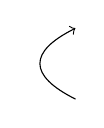
\begin{tikzpicture}[x=3mm,y=3mm]\draw[->] (1,0) .. controls (-1,1) and (-1,2) .. (1,3);\end{tikzpicture}}

\diagram{\deleted{\mbox{\begin{tikzcd}[ampersand replacement=\&,row sep=1ex,column sep=1em,execute at end picture={\draw (current bounding box.south west) rectangle (current bounding box.north east);}]
\unsure{4}\arrow[d,dash] \& \& 1\arrow[d,dash,very thick]\arrow[ddrr,dash,very thick] \& \& \& \text{Leitfaden}\\
\unsure{2} \& \& 2\arrow[d,dash,very thick]\arrow[dl,dash] \& \& \& \\
\& \unsure{5} \& 3\arrow[dr,dash]\arrow[d,dash] \& \deleted{\unsure{2}}\arrow[r,dash] \& 6\arrow[d,dash,thick] \& \\
\& \& \unsure{4} \& 4\arrow[dr,dash] \& \deleted{\unsure{3}} \& \\
\& \& \& \& 7 \&
\end{tikzcd}}}}

\diagram{\begin{tikzcd}[ampersand replacement=\&,row sep=1ex,column sep=1em,execute at end picture={\draw (current bounding box.south west) rectangle (current bounding box.north east);}]
\&1\arrow[d,dash,very thick] \& \& \\
\&2\arrow[d,dash,thick]\arrow[dl,dash]\arrow[ddrr,dash,very thick] \& \& \deleted{\unsure{5|6}}\\
5\&3\arrow[dr,dash]\&\&\\
\&\&4\arrow[dr,dash]\&6\arrow[d,dash,thick]\\
\&\&\&7
\end{tikzcd}}

\margin{\unsure{6.110|6.10}}

% archive sheet number: 32
